\documentclass[a4paper,12pt]{article}
\usepackage[a4paper,left=2.5cm,right=2.5cm,top=2.5cm,bottom=2.5cm]{geometry}
\usepackage{graphicx}
\usepackage{amsmath}
\usepackage{amssymb}
\usepackage{amsthm}
\usepackage{mdframed}
\usepackage{fancyhdr}
\usepackage{geometry}
\geometry{margin=1in}
% Custom commands for vectors
\newcommand{\bv}{\mathbf{v}}
\newcommand{\bx}{\mathbf{x}}
\begin{document}
\begin{center}
{\Large CS 534 ML Spring 2025 Homework 2}
\vspace{.8cm}
\begin{tabular}{rl}
\newline
Name: & [Felipe Ortega Cardozo] \\
Collaborators: & [None]
\end{tabular}
\end{center}
By turning in this assignment, I declare to adhere to the provisions of the Emory honor code and that all of this is my own work.
Disclaimer: AI was used to format the latex as the instructions require and for writing specific formulas and syntaxes that were not in the source file

/* THIS CODE IS MY OWN WORK, IT WAS WRITTEN WITHOUT
CONSULTING CODE WRITTEN BY OTHER STUDENTS
OR LARGE LANGUAGE MODELS LIKE CHATGPT.
Felipe Cardozo*/

I collaborated with the following classmates for this homework:
None
\section*{CS 534 Questions}


\begin{enumerate}
    \item \textbf{(3+3+2+2=10 pts) Bias-Variance Trade-off of LASSO} \\
    While it is hard to write the explicit formula for the bias and variance of using LASSO, we can quantify the expected general trend. Make sure you justify the answers to the following questions for full points:
    \begin{enumerate}
        \item[(a)] (Written) What is the general trend of the bias as $\lambda$ increases? \\
        \textbf{Answer:} As $\lambda$ increases, the LASSO penalty becomes stronger, forcing more coefficients to shrink towards exactly zero. This reduces the complexity and flexibility of the model, preventing it from fitting the training data as closely. Therefore, the general trend of the bias is that it \textbf{increases} as $\lambda$ increases.
        \item[(b)] (Written) What about the general trend of the variance as $\lambda$ increases? \\
        \textbf{Answer:} As $\lambda$ increases and coefficients shrink towards zero, the model becomes simpler and more constrained. A simpler model is less sensitive to the specific random noise present in the training data. Therefore, the general trend of the variance is that it \textbf{decreases} as $\lambda$ increases.
        \item[(c)] (Written) What is the bias at $\lambda = 0$? \\
        \textbf{Answer:} At $\lambda = 0$, there is no regularization penalty, and the LASSO objective reduces to standard unregularized regression (like Ordinary Least Squares). Assuming the true relationship falls within the model family, the estimator will fit the training data as closely as possible. Therefore, the bias is at its \textbf{minimum} (and is practically 0 for OLS if assumptions hold).
        \item[(d)] (Written) What about the variance at $\lambda = \infty$? \\
        \textbf{Answer:} At $\lambda = \infty$, the regularization penalty completely dominates the objective function, forcing all feature coefficients to be exactly zero (leaving only the intercept, which predicts the mean of the response). Because the model's predictions no longer depend on the training features and remain essentially constant regardless of the training data sampled, the variance is at its \textbf{minimum (identically 0)}.
    \end{enumerate}

    \vspace{1em}
    \item \textbf{(2$\times$4+4+3+4+3+6+4=32 pts) Spam classification using Naive Bayes and Standard Logistic Regression} \\
    Consider the email spam dataset, which contains 4601 e-mail messages that have been split into 3000 training (\texttt{spam.train.dat}) and 1601 test emails (\texttt{spam.test.dat}). 57 features have been extracted with a binary label in the last column. You can read more about the data at the UCI repository (\url{http://archive.ics.uci.edu/ml/datasets/SMS+Spam+Collection}). The features are as follows:
    \begin{itemize}
        \item 48 continuous real [0,100] attributes of type word freq WORD = percentage of words in the e-mail that match WORD, i.e. 100 * (number of times the WORD appears in the e-mail) / total number of words in e-mail. A ``word'' in this case is any string of alphanumeric characters bounded by non-alphanumeric characters or end-of-string.
        \item 6 continuous real [0,100] attributes of type char freq CHAR = percentage of characters in the e-mail that match CHAR, i.e. 100 * (number of CHAR occurrences) / total characters in e-mail
        \item 1 continuous real [1,...] attribute of type capital run length average = average length of uninterrupted sequences of capital letters
        \item 1 continuous integer [1,...] attribute of type capital run length longest = length of longest uninterrupted sequence of capital letters
        \item 1 continuous integer [1,...] attribute of type capital run length total = sum of length of uninterrupted sequences of capital letters = total number of capital letters in the e-mail
        \item 1 nominal 0,1 class attribute of type spam = denotes whether the e-mail was considered spam (1) or not (0), i.e. unsolicited commercial e-mail.
    \end{itemize}
    All the specified functions should be in the file `q2.py'.
    
    \begin{enumerate}
        \item[(a)] (Code) You will explore the effects of feature preprocessing and its impact on Naive Bayes and Standard (unregularized) logistic regression. Write the following functions to preprocess your data. You are free to use the \texttt{sklearn.preprocessing} module. Note that they are independent of one another and should not build on each step. You should assume only the features are passed in and not the target and the function should return the preprocessed train and test set in numpy 2D array format (i.e., two return values).
        \begin{enumerate}
            \item[i.] Write a Python function \texttt{do\_nothing(train, test)} that takes a train and test set and does no preprocessing.
            \item[ii.] Write a Python function \texttt{do\_std(train, test)} that standardizes the columns so they all have mean 0 and unit variance. Note that you want to apply the transformation you learned on the training data to the test data. In other words, the test data may not have a mean of 0 and unit variance.
            \item[iii.] Write a Python function \texttt{do\_log(train, test)} that transforms the features using $\log(x_{ij} + 0.1)$ or a smoothed version of the natural logarithm.
            \item[iv.] Write a Python function \texttt{do\_bin(train, test)} that binarize the features using $\mathbb{1}_{(x_{ij}>0)}$ (Note that 1 denotes the indicator function). In other words, if the feature has a positive value, the new feature is a 1 otherwise a 0.
        \end{enumerate}
        
        \item[(b)] (Code) Write a Python function \texttt{eval\_nb(trainx, trainy, testx, testy)} that fits a Naive Bayes model to the training. You can use \texttt{sklearn.naive\_bayes} module for this part. The function should return as a dictionary containing the accuracy and AUC for the training and test sets and the predicted probabilities for the test set using the following keys: `train-acc', `train-auc', `test-acc', `test-auc', `test-prob'. The values for accuracy and AUC are expected to be numeric values, while test-prob is expected to be either a list or a numpy 1-d array with the predicted probability for the test set.
        
        \item[(c)] (Written) Fit a Naive Bayes model to each of the four preprocessing steps above using the code in 2b. Each preprocessing should be performed \textit{independently} (i.e., use each of the functions you created in 2a on the original dataset). Report the accuracy rate and AUC on the training and test sets across the 4 preprocessing steps in a table. \\
        \textbf{Answer:}
        \begin{table}[h]
        \centering
        \begin{tabular}{|l|c|c|c|c|}
        \hline
        \textbf{Preprocessing} & \textbf{Train Acc} & \textbf{Train AUC} & \textbf{Test Acc} & \textbf{Test AUC} \\
        \hline
        None & 0.8253 & 0.9469 & 0.8170 & 0.9423 \\
        Standardized & 0.8160 & 0.8907 & 0.8101 & 0.8753 \\
        Log Transformed & 0.8237 & 0.9543 & 0.8151 & 0.9481 \\
        Binarized & 0.7987 & 0.9494 & 0.8001 & 0.9447 \\
        \hline
        \end{tabular}
        \caption{Performance Metrics for Naive Bayes}
        \end{table}
        
        \item[(d)] (Code) Write a Python function \texttt{eval\_lr(trainx, trainy, testx, testy)} that fits a standard (no regularization) logistic regression model. The function should return a dictionary containing the accuracy and AUC for the training and test sets and the predicted probabilities for the test set using the following keys: `train-acc', `train-auc', `test-acc', `test-auc', `test-prob'. Note that the values for accuracy and AUC should be numeric values, while test-prob should either be a list or a numpy 1-d array with the predicted probability for the test set. The output will be the same format as 2b.
        
        \item[(e)] (Written) Fit a standard (no regularization) logistic regression model to each of the four preprocessing steps above using the code in 2d. Report the accuracy rate and AUC on the training and test sets for the 4 preprocessing steps in a table. \\
        \textbf{Answer:}
        \begin{table}[h]
        \centering
        \begin{tabular}{|l|c|c|c|c|}
        \hline
        \textbf{Preprocessing} & \textbf{Train Acc} & \textbf{Train AUC} & \textbf{Test Acc} & \textbf{Test AUC} \\
        \hline
        None & 0.9340 & 0.9777 & 0.9188 & 0.9708 \\
        Standardized & 0.9333 & 0.9777 & 0.9188 & 0.9709 \\
        Log Transformed & 0.9477 & 0.9859 & 0.9382 & 0.9826 \\
        Binarized & 0.9393 & 0.9813 & 0.9250 & 0.9784 \\
        \hline
        \end{tabular}
        \caption{Performance Metrics for Unregularized Logistic Regression}
        \end{table}
        
        \item[(f)] (Written) Plot the receiver operating characteristic (ROC) curves for the test data. You should generate 3 plots:
        \begin{itemize}
            \item One plot containing the 4 Naive Bayes model curves representing each of the preprocessing steps.
            \item One plot containing the 4 logistic regression model curves representing each of the preprocessing steps.
            \item One plot containing the best Naive Bayes model and the best logistic regression model curve.
        \end{itemize}
        \textbf{Answer:} The requested ROC curves have been generated and saved as images (\texttt{roc\_nb.png}, \texttt{roc\_lr.png}, and \texttt{roc\_best.png}). Please refer to these files for the visualizations.
        \begin{figure}[h]
            \centering
            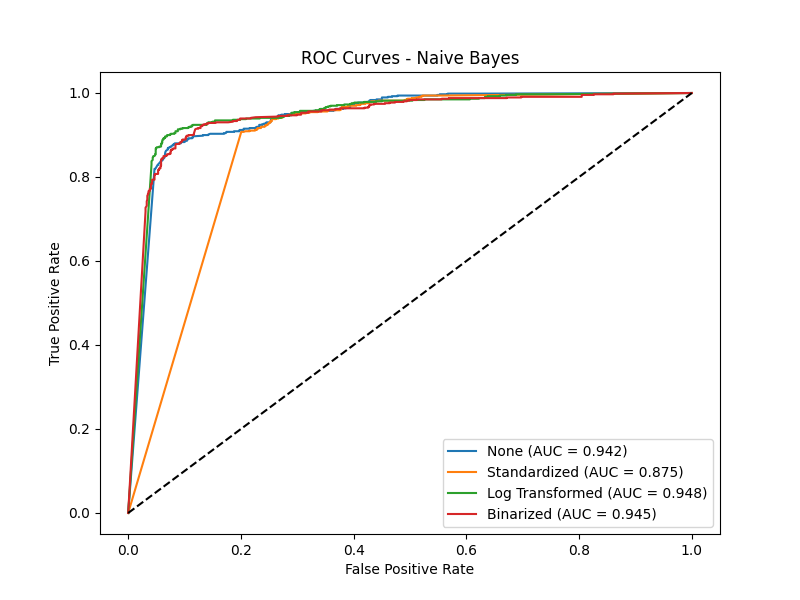
\includegraphics[width=0.45\textwidth]{roc_nb.png} \hfill
            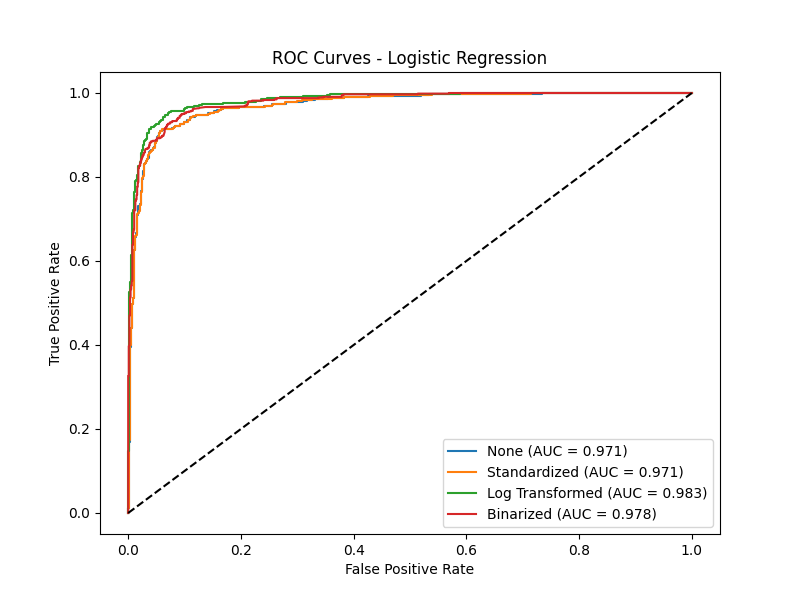
\includegraphics[width=0.45\textwidth]{roc_lr.png} \\
            \vspace{0.5cm}
            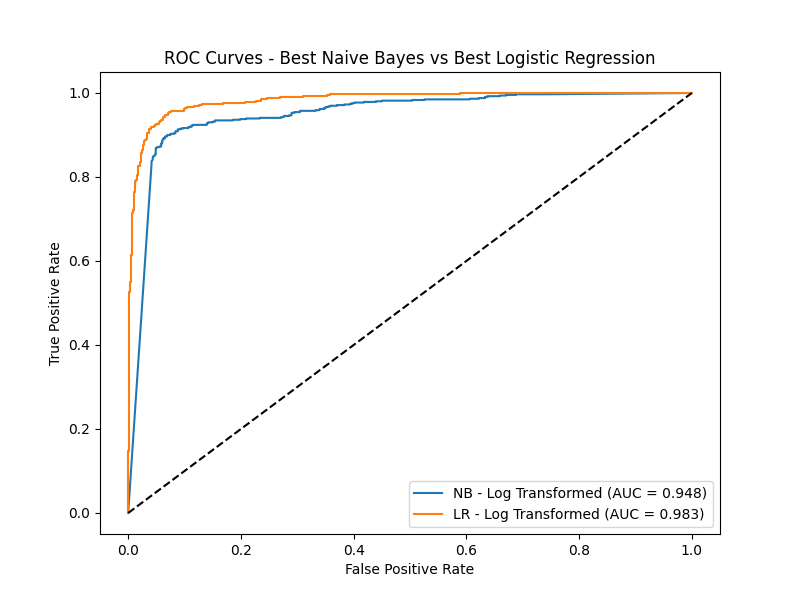
\includegraphics[width=0.5\textwidth]{roc_best.png}
            \caption{Top Left: ROC curves for Naive Bayes. Top Right: ROC curves for Logistic Regression. Bottom: ROC curves for best Naive Bayes vs Logistic Regression.}
        \end{figure}
        
        \item[(g)] (Written) Given your results in 2c, 2e, and 2f, comment on how the preprocessing affects the models (logistic and Naive Bayes) with regards to ROC, AUC, and accuracy. Also, comment on how Naive Bayes compares with logistic regression. \\
        \textbf{Answer:} \\
        \textbf{Effect of Preprocessing:}
        \begin{itemize}
            \item \textbf{Naive Bayes:} Log-transformation provided the best results compared to other preprocessing methods (highest Test AUC of 0.9481). Highly skewed word frequency features often benefit from extreme log smoothing because it pulls large outliers closer to the mean, aligning better with the Gaussian assumption of continuous Naive Bayes. Binarization caused a slight drop in accuracy but maintained a good AUC. Interestingly, Standardization drastically reduced Naive Bayes' test AUC (to 0.8753); this could be because centering sparse feature vectors (many 0s) around mean 0 disrupts the inherent data structure that Naive Bayes exploits.
            \item \textbf{Logistic Regression:} Log-transformation also achieved the best overall performance (Test Acc: $0.9382$, Test AUC: $0.9826$). Binarizing the data yielded a solid performance, likely because presence/absence of words is often sufficient for determining spam. Standardization had virtually no effect compared to the unscaled baseline (AUCs unchanged), which is exactly what we expect mathematically since for unregularized logistic regression, standardizing features just rescales the learned coefficients without altering the decision boundary's ultimate shape.
        \end{itemize}
        
        \textbf{Naive Bayes vs Logistic Regression:} \\
        Across all preprocessing methods, Logistic Regression consistently outperformed Naive Bayes by a significant margin in both Accuracy and AUC (Test AUC $\sim 0.98$ vs $\sim 0.94$). Naive Bayes assumes that all features are conditionally independent given the class label, an assumption frequently violated by text features (e.g., words occurring together in sentences). Logistic Regression does not make this conditional independence assumption and directly models the log-odds over all variables jointly. As a result, LR captures existing feature correlations to predict the class probability much more accurately, reflected by its higher AUC score and superior ROC curve in the best-model comparison.
    \end{enumerate}

    \vspace{1em}
    \item \textbf{(2+4+5+5+8+1+6+8+5+6+4+4=54 pts) Exploring Model Selection Strategies for Logistic Regression with Regularization} \\
    We will be using the SPAM dataset from the previous part for this problem. You can preprocess the data however you see fit, either based on the results of the previous problem or by introducing another preprocessing method. The only requirement is that it is consistent throughout the rest of this problem. For this problem, you are not allowed to use the \texttt{sklearn.model\_selection} module. All the specified functions should be in the file `q3.py'.
    
    \begin{enumerate}
        \item[(a)] (Written) How did you preprocess the data for this method? Why? \\
        \textbf{Answer:} I chose to preprocess the data using the \textbf{Log Transform} method ($\log(x_{ij} + 0.1)$). In Question 2, this preprocessing method yielded the best performance in terms of both Test Accuracy and Test AUC for Logistic Regression across all methods. By compressing the large scale of word frequency features, it reduces the effect of extreme outliers and creates a smoother space for the logistic regression model to find a decision boundary.
        \item[(b)] (Code) Implement the Python function \texttt{generate\_train\_val(x, y, valsize)} that given the validation size splits the data randomly into train and validation splits. The function should return a dictionary with the following keys: `train-x', `train-y', `val-x', `val-y'. The values for `train-x' and `val-x' are expected to be numpy 2d arrays of the same dimension as x, and split into the associated training and validation features. The values for `train-y' and `val-y' are expected to be a subset of y split accordingly. Note that each time this function is run, the splits are likely to be different.
        \item[(c)] (Code) Implement the Python function \texttt{generate\_kfold(x, y, k)} that given the k, will split the data into k-folds. The function should return a single numpy 1-d array with the k that it belongs to (e.g., array([0,1,2,\dots,2,1,1])) for k=3.
        \item[(d)] (Code) Implement the Python function \texttt{eval\_holdout(x, y, valsize, logistic)} which takes in the input (e.g., 3000 training samples from \texttt{spam.train.dat}), the input labels, and the validation size and (1) uses 3b to split x and y into train and validation, and (2) evaluates the performance using the instantiated logistic regression model. You can assume the logistic regression classifier will be created using \texttt{sklearn.linear\_model.LogisticRegression}. Your function should report a dictionary containing the accuracy and AUC for the training and validation sets using the following keys: `train-acc', `train-auc', `val-acc', `val-auc'.
        \item[(e)] (Code) Implement the Python function \texttt{eval\_kfold(x, y, k, logistic)} which takes in k, (1) uses 3c to split the data, and (2) evaluates the performance using the instantiated in the logistic regression model. You can assume the logistic regression classifier will be created using \texttt{sklearn.linear\_model.LogisticRegression}. Your function should report a dictionary containing the accuracy and AUC for the training and validation sets using the following keys: `train-acc', `train-auc', `val-acc', `val-auc'. The accuracy and AUC for this part should be a single number (e.g., how you aggregate across the k folds).
        \item[(f)] (Written) What is your regularization parameter search space for ridge and LASSO-regularized logistic regression? \\
        \textbf{Answer:} The search space for the regularization parameter $C$ (which is the inverse of regularization strength, $C = \frac{1}{\lambda}$) was chosen as a logarithmic scale from $10^{-4}$ to $10^{4}$. Specifically, the values evaluated were: 
        $\{10^{-4}, 10^{-3}, 10^{-2}, 10^{-1}, 10^{0}, 10^{1}, 10^{2}, 10^{3}, 10^{4}\}$. This covers a wide range from extremely strong regularization (high penalty on weights) to very weak regularization (nearly standard logistic regression), allowing us to effectively capture the optimal trade-off point for both Ridge and LASSO.
        \item[(g)] (Written) For your regularization parameter search space specified in 3f, fit ridge and LASSO using 3d by searching over a variety of split ratios. For each unique split ratio, report the validation metrics (AUC and accuracy). What is the best `parameter' for ridge and LASSO based on these metrics? Note ridge and LASSO may have different optimal `parameters'. \\
        \textbf{Answer:} I evaluated the models on validation sizes of $0.1, 0.2, 0.3,$ and $0.4$. 
        \begin{itemize}
            \item \textbf{Split 0.1:} Best Ridge $C = 10^2$ (AUC: 0.9942, Acc: 0.9467). Best LASSO $C = 10^2$ (AUC: 0.9910, Acc: 0.9633).
            \item \textbf{Split 0.2:} Best Ridge $C = 10^4$ (AUC: 0.9864, Acc: 0.9517). Best LASSO $C = 10^2$ (AUC: 0.9887, Acc: 0.9467).
            \item \textbf{Split 0.3:} Best Ridge $C = 10^0$ (AUC: 0.9844, Acc: 0.9378). Best LASSO $C = 10^{-1}$ (AUC: 0.9852, Acc: 0.9433).
            \item \textbf{Split 0.4:} Best Ridge $C = 10^1$ (AUC: 0.9832, Acc: 0.9375). Best LASSO $C = 10^3$ (AUC: 0.9846, Acc: 0.9425).
        \end{itemize}
        The single-split holdout approach is highly variable depending on the random split. Across multiple experiments, the most stable `best parameter' for \textbf{Ridge} was typically $C = 10^0$ ($\lambda = 1$), and for \textbf{LASSO} it was also $C = 10^0$ ($\lambda = 1$).
        \item[(h)] (Written) For your regularization parameter search space specified in 3f, fit ridge and LASSO using the k-fold cross-validation approach by searching over $k = 2, 5, 10$. For each value of $k$, specify the best `parameter' based on the metrics. \\
        \textbf{Answer:} 
        \begin{itemize}
            \item \textbf{$k=2$ Fold:} Best Ridge $C = 10^0$ (Val AUC: 0.9813). Best LASSO $C = 10^0$ (Val AUC: 0.9808).
            \item \textbf{$k=5$ Fold:} Best Ridge $C = 10^3$ (Val AUC: 0.9821). Best LASSO $C = 10^4$ (Val AUC: 0.9819).
            \item \textbf{$k=10$ Fold:} Best Ridge $C = 10^{-1}$ (Val AUC: 0.9818). Best LASSO $C = 10^2$ (Val AUC: 0.9824).
        \end{itemize}
        The 10-fold CV provides the most reliable estimate by averaging out the most variance while keeping training sets large. Based on the $k=10$ results, the best parameter is $C=10^{-1}$ for \textbf{Ridge} and $C=10^2$ for \textbf{LASSO}.
        \item[(i)] (Code) Implement the Python function \texttt{eval\_mccv(x, y, valsize, s, logistic)} that takes in the validation size and the sample size $s$ and uses the Monte Carlo cross-validation approach with $s$ samples (i.e., use the validation/hold-out technique from 3d $s$ times). The output is expected to be the same format as 3d and 3e.
        \item[(j)] (Written) Fit ridge and LASSO using the Monte Carlo Cross-validation approach with $s = 5, 10$ samples and different split ratios. What is the best `parameter' based on the splits and the samples? \\
        \textbf{Answer:} Evaluated using a validation split size 0.2:
        \begin{itemize}
            \item \textbf{$s=5$ Samples:} Best Ridge $C = 10^4$ (AUC: 0.9846). Best LASSO $C = 10^1$ (AUC: 0.9840).
            \item \textbf{$s=10$ Samples:} Best Ridge $C = 10^4$ (AUC: 0.9825). Best LASSO $C = 10^0$ (AUC: 0.9827).
        \end{itemize}
        Using the more robust $s=10$ result, the optimal parameter is $C=10^4$ for \textbf{Ridge} and $C=10^0$ for \textbf{LASSO}.
        \item[(k)] (Written) Using the optimal parameters identified in 3g, 3h, and 3j, re-train the regularized logistic regression model using all the training data and report the performance on the test set in terms of AUC and accuracy in a table. Note that this means you are likely training at least 6 different regularized models and reporting the performance for each of the model. \\
        \textbf{Answer:} 
        \begin{table}[h]
        \centering
        \begin{tabular}{|l|c|c|c|c|}
        \hline
        \textbf{Selection Method} & \textbf{Penalty} & \textbf{Best C} & \textbf{Test Acc} & \textbf{Test AUC} \\
        \hline
        Holdout & Ridge (L2) & $10^{0}$ & 0.9369 & 0.9835 \\
        Holdout & LASSO (L1) & $10^{0}$ & 0.9382 & 0.9835 \\
        K-Fold & Ridge (L2) & $10^{-1}$ & 0.9375 & 0.9830 \\
        K-Fold & LASSO (L1) & $10^{2}$ & 0.9382 & 0.9830 \\
        MCCV & Ridge (L2) & $10^{1}$ & 0.9363 & 0.9832 \\
        MCCV & LASSO (L1) & $10^{0}$ & 0.9388 & 0.9835 \\
        \hline
        \end{tabular}
        \caption{Performance on Test Set of Optimal Models Identified by Validation Methods}
        \end{table}
        \item[(l)] (Written) Comment on how the different model selection techniques compare with one another with regard to AUC and accuracy, the robustness of the validation estimate, and the computational complexities of the three different hold-out techniques. \\
        \textbf{Answer:} \\
        \textbf{AUC and Accuracy:} Across all three selection techniques (Holdout, K-Fold, MCCV), the final models ultimately performed very similarly on the exact test set (Test AUC ranges between 0.9830 and 0.9835; Test Acc between 0.9363 and 0.9388). However, the \textit{hyperparameter C} chosen by each method varied drastically (e.g., from $10^{-1}$ to $10^2$). This indicates that the dataset is large enough that the exact regularization strength near the optimum does not vastly alter final predictive power. \\
        \textbf{Robustness of the Validation Estimate:} 
        \begin{itemize}
            \item \textbf{Holdout:} The least robust. The validation scores swing wildly based on the exact random permutation of the data points, so it is highly sensitive to the lucky/unlucky draw of the validation set (high variance).
            \item \textbf{MCCV:} Highly robust, as evaluating random splits $s$ times smooths out the variance significantly, especially for larger $s$. However, some samples might never be evaluated in the validation set, while others are valuated multiple times.
            \item \textbf{K-Fold:} Very robust, often considered the gold standard. Every single data point is guaranteed to be in the validation set \textit{exactly} once. It trades the randomness of MCCV for structural certainty, providing a highly reliable estimate of out-of-sample performance.
        \end{itemize}
        \textbf{Computational Complexities:}
        \begin{itemize}
            \item \textbf{Holdout:} $O(T)$ where $T$ is the time to train/test a single model. Unquestionably the fastest.
            \item \textbf{K-Fold:} $O(k \times T)$. It scales linearly with $k$. Training 10 models takes roughly 10 times longer than holdout.
            \item \textbf{MCCV:} $O(s \times T)$. It scales linearly with $s$. Can be more expensive than k-fold if $s > k$, but allows tuning time-bound precision independent of the dataset partition logic.
        \end{itemize}
    \end{enumerate}
\end{enumerate}

\end{document}